\section{\textcolor[HTML]{D32F2F}{Kravspesifikasjon}}
\label{kravspesifikasjon}

Dette kapitlet vil ta for seg aktiviteter gruppen gjorde i tjenestedesign som basis for å danne krav for applikasjonen.

\subsection{Tjenestedesign}
\label{tjenestedesign}
Tjenestedesign handler om å skape gode brukeopplevelser sett fra brukeres perspektiv. For å få en overordnet forståelse for hvilke kvaliteter et produkt bør ha for å skape brukevennlighet, er det viktig å se \textit{styrken} en app kan ha, \textit{nytten} den gir og \textit{tjenesten} man kan få ut av produktet. Dersom disse tre faktorene er nært knyttet sammen og gjør at en bruker blir fristet til å ta i bruk produktet, vil produktet ha stor suksess og man kan si at en tjeneste og produkt blir en side av samme sak. Et eksempel på dette er \textit{Apple iPod} og musikk, der man med et produktfokus ser på iPod som en direkte kobling mot musikk, og med et tjenestefokus ser på musikk en direkte kobling mot iPod\cite{servicedesign}.
\\\\
De ulike aktivitetene som presenteres i dette kapitlet vil først bli presentert i generell form, så vil det bli gitt en forklaring på hvordan gruppen utførte den enkelte aktivitet i prosjektet. Dette blir gjort for å gi leseren oversikt over temaet før videre utdyping. 

\subsubsection{Segmentering og målgrupper}
Et segment betyr \textit{del av noe}, og innebærer å dele opp et marked i flere interesseområder. Målgrupper relaterer seg som grupper av personer med fellestrekk innenfor kjønn, alder, interesser, bosted, utdanning eller lignende\cite{malgruppe}. Ved å velge en spisset målgruppe og se den i sammenheng med et segment kan man drive mer målrettet og treffsikker markedsføring, eller konseptutvikling i dette tilfellet\cite{malgruppe2}.
\\\\
Gruppen besøkte Sirkus shopping og gjorde observasjon av handlemønster blant personer inne på senteret. Ut fra dette feltstudiet fikk gruppen en god oversikt og kunne foreta en segmentering av handlemønster og analysere hvilke målgrupper som befant seg på senteret. 
Gjennom feltstudiet knyttet gruppen målgruppene opp mot segmenteringen, se Tabell \ref{tab:segmenterogmålgrupper}, og valgte travle mødre og fedre som segment og målgruppe. Grunnen til denne beslutningen var at det var disse gruppene som var mest framtredende under observasjonen og noe gruppen syntes var interessant å utforske videre.

\begin{table}[H]
    \caption{Segmenter og målgrupper}
    \label{tab:segmenterogmålgrupper}   
    \centering
    \begin{tabular}{|L{5em} L{15em} L{22em}|}
    \hline
        \rowcolor[HTML]{D32F2F}
        \textbf{\textcolor{white}{Segmenter}} & \textbf{\textcolor{white}{Målgrupper}} &
        \textbf{\textcolor{white}{Beskrivelse}}\\
        \rowcolor[HTML]{E6E6E6}
        Travle & Mødre, fedre, menn, forretningspersoner & Målrettede handlere som er raske mellom butikker \\
        Fingåere & Mødre, unge/ungdommer, Kvinner, Eldre & Noen har et mål andre ikke. Går rolig gjennom senteret, uten å stresse \\
        \rowcolor[HTML]{E6E6E6}
        Hengere & Unge/ungdommer & Ingen mål. Er på senteret for det sosiale \\
        Sittere & Unge/ungdommer, menn, fedre, eldre, mødre & Ønsker å møte folk, eller er med andre på handletur\\
        \hline
    \end{tabular}
\end{table}

\subsubsection{Personas}
Personas er oppdiktede karakterer som skal representere en målgruppe og et markedssegment\cite{feltstudie}. Oppgaven til en personas er å representere målet og oppførselen til den spesifikke målgruppen. Dette er nyttig når det kommer til avgjørelser angående design, interaksjon og egenskapene til produktet. Ved å gi målgruppen et ansikt, vil det hjelpe utviklerne av produktet med å relatere seg mer brukerne, og få mer empati\cite{preece}.
\\\\
Gruppen valgte å fokusere på travle småbarnsforeldre, ut fra resultater gjort etter segmentering og målgruppeanalyse i Tabell \ref{tab:segmenterogmålgrupper}. På bakgrunn av dette endte gruppen opp med Roar og Trude som skal representere travle foreldre av begge kjønn, med barn i forskjellige aldre. Disse personasene ble laget med programmet Xtensio, der gruppen bestemte personlighet, mål, frustrasjoner og motivasjon som var typisk for denne brukergruppen. I figur \ref{fig:personasTrude} er Trude Pettersen presentert, mens i figur \ref{fig:personasRoar} er Roar Johnsen presentert.

\noindent\textbf{Scenario: Trude på handletur}\\
Trude er en 33 år gammel dame som jobber som lærer. Hun har to barn, Tina og Thomas, og er gift med Trond. På fritiden liker Trude å gå tur i skog og mark, bake og sy. Hun jobber som klasseforstander for en 4. klasse ved Strinda barneskole, og trives godt i jobben sin. Sønnen til Trude, Thomas, trenger nye fotballsko, pluss at Tina skal i fødselsdag på lørdag og må finne en presang hun kan gi venninnen. Trude tar dermed med seg begge barna på Sirkus shopping slik at de kan få ordnet begge deler samtidig. 
\\\\
Når de kommer fram på Sirkus shopping parkerer Trude bilen i parkeringshuset og leier ungene inn på senteret. Tina vil veldig gjerne inn i lekebutikken for å se på dukkene, men Trude må si nei og si at de først skal finne fotballsko til Thomas. De går inn på MX Sport og får hjelp av en av de ansatte. Tina synes det er ganske kjedelig å se på storebroren prøve sko, og begynner å gå rundt i butikken for å se om hun finner noe hun kan leke med. Trude kan ikke underholde begge to samtidig og tenker det går fint om Tina får bort og ser på de rosa jentesyklene borte i hjørnet. Thomas bestemmer seg til slutt for et par røde fotballsko med svarte striper. Trude betaler i kassen og Tina kommer etter. Hun forteller moren at hun må tisse, og de må dermed finne det nærmeste toalettet. Thomas får i oppgave å bære posen med fotballskoene, og kan vente i Fotballbutikken mens Tina og Trude går på toalettet.

\begin{figure}[H]
    \begin{figure}
    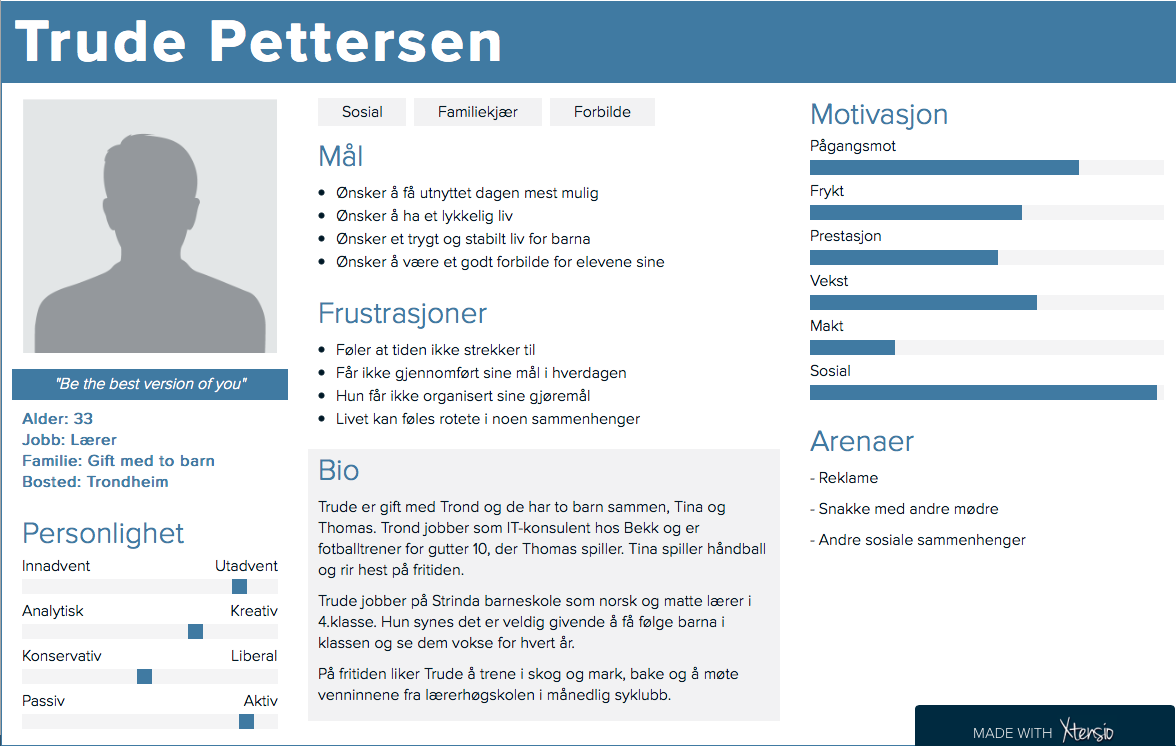
\includegraphics[scale=0.28]{images/personas/personasTrude}
    
\includegraphics[scale=0.27]{images/personas/trude}
    \caption{Personas av småbarnsmor Trude}
    \label{fig:personasTrude}
    \end{figure}
\end{figure}

\noindent\textbf{Scenario: Roar er alene hjemme}\\
Roar er en 45 år gammel mann som jobber som ingeniør. Han bor i Trondheim, og er gift med Ingunn. Hun jobber som flyvertinne. Sammen har de to barn, Ingrid og Martin. På fritiden liker Roar å gå tur i skog og mark, men får ikke så mye tid til dette fordi Ingunn ofte er bortreist i jobbsammenheng og begge barna er i tenårene. De krever tett oppfølging, og Roar bruker mye tid på leksehjelp, kjøring av barna og husarbeid. 
\\\\
Ingrid fyller snart år, og Ingunn har planlagt bursdagsfest for datteren. Hun skal feire hjemme, og Ingunn har satt opp en handleliste. Selskapet skal være lørdag kveld, og Ingunn hadde planlagt å handle torsdag kveld. Onsdag formiddag får hun en telefon fra jobben med spørsmål om hun kan ta en ekstra vakt siden en av kollegene har blitt syke. Ingunn sier ja, og ber Roar ta ansvar for å handle inn til fødselsdagen. Han er ikke så veldig komfortabel med å reise på Sirkus shopping. Han synes det er litt uoversiktlig med mange butikker, og det er tross alt Ingunn som pleier å handle. Han vet heller ikke helt hva Ingrid har lyst til å ha på festen sin, siden kona kun har skrevet ting som “brus” og “kake” og ikke spesifisert helt hva han skal kjøpe.

\begin{figure}[H]
    \begin{figure}
    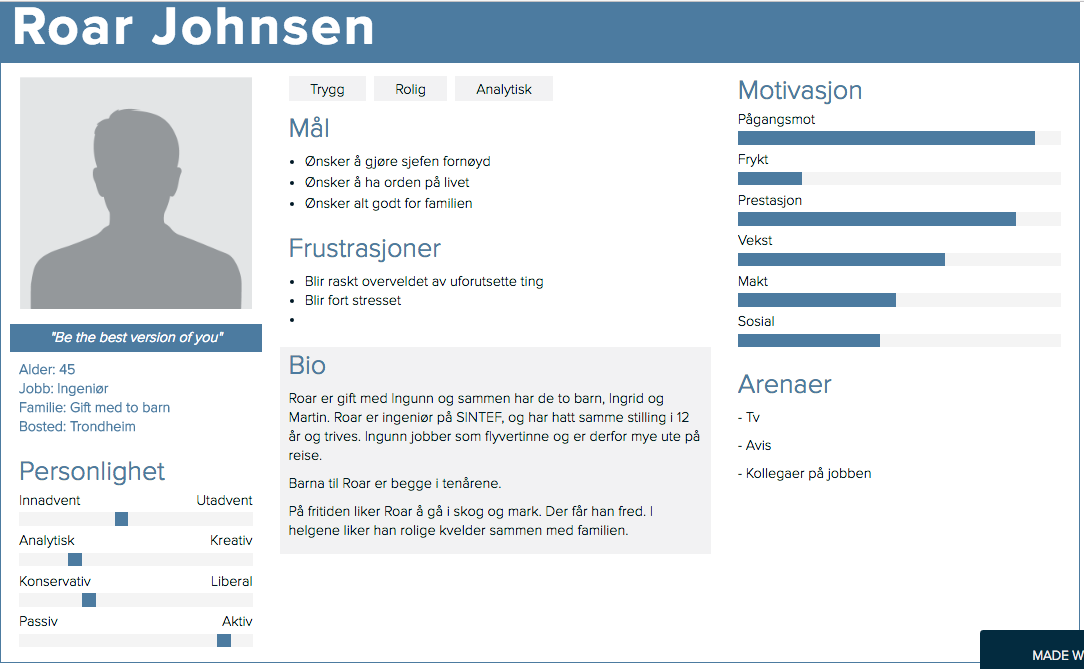
\includegraphics[scale=0.3]{images/personas/personasRoar}
    
\includegraphics[scale=0.25]{images/personas/roar}
   
    \caption{Personas av tenåringsfar Roar}
    \label{fig:personasRoar}
    \end{figure}
\end{figure}

\subsubsection{Spørreundersøkelse}
Spørreundersøkelser er en veletablert teknikk for å samle demografisk data og meninger fra brukere\cite[s.~244]{preece}. Spørreundersøkelsene kan ha åpne eller lukkede spørsmål, avhengig av hva man ønsker å finne ut. Det viktige når man gjør spørreundersøkelser er å stille de riktige spørsmålene. De skal ikke lede brukeren på vei, slik at de svarer det man ønsker å høre. Spørsmålene som stilles må være nøytrale, og la brukeren selv gjøre seg opp en mening om temaet.
Spørreundersøkelser kan struktureres på mange måter. Noen spørsmål kan være åpne, for eksempel med tekstfelt hvor brukeren kan skrive inn sitt eget svar. Andre spørsmål kan bestå av svaralternativer, det brukeren skal velge ett eller flere alternativ som de mener er best. Et eksempel kan være demografiske spørsmål\cite[s.~245]{preece}. Brukeren kan velge kjønn, blant to alternativer (mann, kvinne). Det kan også spørres om alder, hvor brukeren skal velge ett alternativ blant flere; 10-15, 16-20, 21-25, 26-30 osv. Man kan også lage skalaer hvor brukeren kan rangere svaret sitt. Her er det vanlig å enten bruke tallene en til fem, eller "sterkt enig" til "sterkt uenig".
\\\\
Undersøkelsen gruppen lagde hadde fokus på å finne ut demografi og behov til brukerne av kjøpesentre, og da spesielt Sirkus shopping. Spørreundersøkelsen ble laget i \textit{Google Forms}, som er en gratis digital tjeneste for spørreskjemaer. Her legger man inn spørsmål, og kan velge mellom flere svarformer som f.eks. ett svar, flere svar eller åpne tekstfelt. Undersøkelsen deles med en link til brukerne, og svarene kan så enten vises grafisk med diagrammer eller som rådata i \textit{Microsoft Excel} regneark. Dette gjorde det svært enkelt for gruppen å dele undersøkelsen og analysere resultatene i ettertid. Resultatene fra spørreundersøkelsen, med spørsmålene som ble stilt, er vedlagt i Appendix \ref{App:AppendixA}.
\\\\
Det gruppen kunne se ut fra de 51 svarene som de fikk på spørreskjemaet var i hovedsak at de aller fleste (98\%) hadde smarttelefon (se Figur \ref{fig:smarttelefon}), og dersom dette gjenspeiler kjøpesenterets brukergruppe ellers så vil de aller fleste kundene kunne ta i bruk en app. 41,5 prosent av brukerne svarte at de var på shopping 2-4 ganger i måneden (se Figur \ref{fig:shopping}), mens 25,5 prosent svarte de var på shopping kun én gang i måneden. Nesten sytti prosent av brukerne svarte at de har et spesifikt mål med handleturen (se Figur \ref{fig:formal}), mens litt under femti prosent svarer at de går i butikkene for å titte. En gjenganger blant svarene på hva som irriterer brukerne når de oppholder seg på senteret er at det er for mye mennesker (54,9\%), at de ikke finner ønsket produkt (56,9\%) og at senteret er uoversiktlig (37,3\%) (se Figur \ref{fig:irritasjonsmoment}). Nesten 61 prosent av de spurte har aldri brukt en app for å forbedre handleopplevelsen, mens noen nevner apper som Mattilbud, Prisjakt og Zalando. Videre svarer 72,5 prosent at de gjerne hadde brukt en slik app dersom det fantes (se Figur \ref{fig:brukeapp}), og det tolket gruppen som at brukerne var positive til at det ble utviklet en app for formålet. Til slutt ble det spurt om brukerne hadde et forslag til hva en slik app kunne inneholde. Da kom det forslag om blant annet lagerbeholdning, pris på varer, butikkoversikt, tilbud, rabatter og strekkodescanner. Dette vare noe gruppen tok med seg i utvikling av konseptet.
\\\\
Det må nevnes at spørreundersøkelsen antakeligvis ikke har et representativt utvalg. Undersøkelsen ble sendt på nett, og distribuert i nettverket til de fire gruppemedlemmene. Det betyr at man ikke har nådd de som for eksempel ikke har Internett tilgjengelig, eller at man har kun nådd spesielle grupper fordi gruppen ikke har bredt nok nettverk. Antall svar på undersøkelsen er også forholdsvis få, men gruppen valgte likevel å bruke resultatene de fikk. 

% \textbf{Intervjuer} kan sies å være en samtale med en mening\cite{kahn}. Hvordan et intervju gjøres avhenger av intervjueren. Noen intervju kan flyte som en vanlig samtale, mens andre intervju kan være styrt av forhåndsbestemte spørsmål. Man kan si at det finnes fire hovedtyper av intervjuer: ustrukturerte, strukturerte, semi-strukturerte og gruppeintervjuer

% Vi har vell ingen intervjuer å referere til????
% \\\\
% \cite[s.~233]{preece}. De første tre beskriver hvor mye intervjueren styrer samtalen, mens den siste beskriver en gruppe som ledes av en intervjuer. 
\subsubsection{Brukeropplevelse}\\
Brukeropplevelsen er viktig når man jobber med interaksjonsdesign. Brukeropplevelse beskrives som hvordan et produkt oppfører seg og blir brukt av personer i den virkelige verden\cite[s.~12]{preece}. Ethvert produkt som brukes av noen har en brukeropplevelse, eller UX som det forkortes på engelsk. Brukeropplevelse kan ikke designes, men man kan legge til rette for en god brukeropplevelse. Ved å analysere brukernes behov kan man få et bedre resultat enn hvis man setter i gang arbeidet med å utvikle noe uten å ha snakket med sluttbrukerne.
\\\\
Brukbarheten til et produkt kan måles, ved å se på seks punkter som peker på ulike mål. Disse listes gjerne opp som spørsmål, og målet er å gi interaksjonsdesigneren bekreftelse på om produktet er brukervennlig eller ikke \cite[s.~19]{preece}. De seks punktene man ser på er hvor effektivt noe er å bruke(\textit{effectiveness}), hvor raskt det er å bruke (\textit{efficiency}), hvor trygt det er å bruke (safety), hvor nyttig det er (\textit{utility}), hvor enkelt det er å lære (\textit{learnability}), og hvor enkelt det er å huske (\textit{memorability}). Alle disse punktene er det lurt å ha i tankene når produktet utvikles, for å så ta de fram igjen når produktet skal testes.
%skrive noe om behovene

\subsubsection{Konseptet}
\label{konseptet}

Gruppen ville lage en applikasjon som skulle forenkle og effektivisere shoppingopplevelsen til travle småbarnsforeldre. Gruppen kom opp med en idé om en app hvor man har en virtuell handlekurv med alle produktene man ønsker å kjøpe. Når kunden finner et produkt hun eller han ønsker å kjøpe, scanner kunden en RFID i prislappen som gjør at produktet dukker opp i appen og kan legges i handlekurven. Inspirert av skanningen fra Zalando sin applikasjon, se Kapittel \ref{zalando}. I appen velger kunden størrelse, og kan endre antall. I den virtuelle handlekurven vil kunden se en oversikt over produkter hun eller han har valgt seg ut, samt en totalsum på varene, inspirert fra både Zalando og Boozt sin handlekurv, se Kapittel \ref{lignendeApper}. 
\\\\
Når kunden på slutten av handleturen ønsker å betale og ta med seg varene hjem vil ordren sendes til utleveringsstedet og kunden betaler for varene. Dette kan enten gjøres i appen, eller ved utleveringsstedet for kunder som ikke har aktivert betalingstjenester på smarttelefonen sin. Dersom kunden ikke vil handle varene med en gang, kan de legges til i en ønskeliste og lagres til senere. For eksempel kan en student gå rundt på senteret og legge produkter til i sin ønskeliste, og før jul dele denne med bestemor eller onkel slik at de kan gå inn på senteret og handle riktig produkt og størrelse uten problem.
\\\\
Dette forenkler shoppingsopplevelsen ved å samle alle kjøp på én handleliste på smarttelefonen til brukerne. Effektiviseres ved å ha betalingsløsning på appen,
fjerner kassene i butikken og gir muligheten til å hente alle de kjøpte varene ferdig pakket i en ekstern henteavdeling (slik som på IKEA og SmartClub). Bra for travle småbarnsfamilier som ikke har muligheten til å bære alle kjøp samtidig som de har barn med, og sparer dem tid ved å kunne forhåndslage lister og gå direkte til henteavdeling.

\subsubsection{Ideen bak produktet}
Gjennom observasjoner og intervjuer så gruppen det at det var et ønske om en enklere handleopplevelse. Mange kunder opplever det som slitsomt å måtte bære rundt på varene de hadde kjøpt, og noen ønsket også å kunne se alle typer av et produkt før de bestemte seg for hvilken de ville kjøpe. Eksempelvis var det noen kunder som ønsket å kunne se alle genserne på senteret før de kjøpte en av dem. De ønsket ikke å gå innom flere butikker som hadde noe av det samme utvalget, men heller se og prøve alle genserne på samme sted.
\\\\
Dette konseptet effektiviserer handeturen til målgruppen ved at brukeren kan registrere varer fra forskjellige butikker, for så å hente alle varer sammen på varelageret. Betaling via appen gjør at brukeren unngår betalingskø i kassen. Delingsfunksjonen gjør det mulig å sende ønskelister til andre brukere av appen, som da kan gå direkte til varelageret for å hente ut varene i listen. Løsningen er også hensiktsmessig for målgruppen, småbarnsforeldre, som ofte ikke har nok hender til å passe på barn samtidig som de må bære rundt på alle varene de skal kjøpe.
\\\\
Et annet punkt som ble nevnt av intervjuobjektene var oversiktlighet på senteret. Mange sentre har en infotavle, men det er få som tar seg tid til å studere denne nøye. Få sentre er også lagt opp slik at butikker i samme kategori ligger ved siden av hverandre. Intervjuobjektene fortalte at det kunne være vanskelig å finne fram til butikkene de ville besøke dersom de hadde lite tid, og ønsket en løsning på dette. 
\\\\	
For å løse punktet om navigasjon inne på senteret kom gruppen opp med en idé om å ha streker på gulvet som indikerer en rute man kan følge. Det kan for eksempel være å ha en grønn rute for herrer. Da er det en linje i gulvet som går innom alle butikker som herrer har interesse for på senteret, som for eksempel klesbutikk for menn. Tilsvarende kan man ha en rute for sport, som går innom sportsbutikker på senteret. Disse rutene går det også an å ha tilpasset sesong. Rundt skolestart kan det for eksempel legges opp en rute som går innom alle butikkene hvor man kan handle ting til skolestart. For eksempel bokhandel, sportsbutikk og klesbutikk. Denne ideen gikk ikke gruppen videre med i dette prosjektet, men kunne vært realisert i varehuset dersom modellen hadde blitt tatt i bruk.
\\\\
Etter å ha landet på en produktidé tok gruppen kontakt med Sirkus shopping igjen for å få svar på noen sprøsmål. Gruppen lurte på om butikkene på senteret er plassert på en spesiell måte, eller om de er plassert etter hva som er ledig når en butikk vil etablere seg. På dette svarte senterlederen at butikkene er plassert etter butikkenes egne ønsker og arealutforming. Gruppen hadde også spørsmål angående samlokalisering av bransjer. Under feltstudiene la gruppen merke til at f.eks. skobutikkene ikke lå ved siden av hverandre. Her kunne senterlederen opplyse om at bransjer gjerne vil ligge ved siden av hverandre siden de drar nytte av dette. Det er viktig med et større utvalg i enkelte bransjer som tekstil, sko, reiseeffekter, gullsmed og spisteder. Dette underbygger gruppens idé om å samle alle gensere ett sted, og alle joggesko et annet sted.

\subsubsection{Kundereiser}
\label{sec:kundereise}
Kundereiser, eller \textit{customer journeys}, er grafiske framvisninger med utgangspunkt i ulike synspunkt av hvordan et system oppfører seg i en gitt prosess\cite{servicedesign}. De ulike synspunktene/perspektivene blir sett på som ulike kunder av systemet, med ulike formål. I en slik framvisning vil en prosess, \textit{lifecycle stages}, identifisere kundens berøringspunkter, \textit{touchpoints}, mot systemet, samt kundes tanker og overordnede opplevelse gjennom hele prosessen. Ved å lage kundereiser får man større forståelse for de ulike kundenes behov og kan gjøre det enklere å definere funksjoner som systemet må inneholde\cite{servicedesign}.
\\\\
I prosjektet identifiserte gruppen tre ulike kunder, med interesse i og bruk for i applikasjonen. Kunden på senteret, den ansatte i de 128 butikkene og den ansatte på lageravdelingen på Sirkus shopping. For å presentere dem valgte gruppen å ha en statisk livssyklus blant alle kundene, da alle tilknyttes samme prosess gjennom bruken av applikasjonen. Derimot ble berøringspunktene, tankene og humøret forskjellig, da de har ulike roller og oppgaver i en handleprosess. I Figur \ref{fig:customerKunde}, Figur \ref{fig:customerAnsatt}, og Figur  \ref{fig:customerLager} vises hver av disse perspektivene presentert som en kundereise. 

\begin{figure}[H]
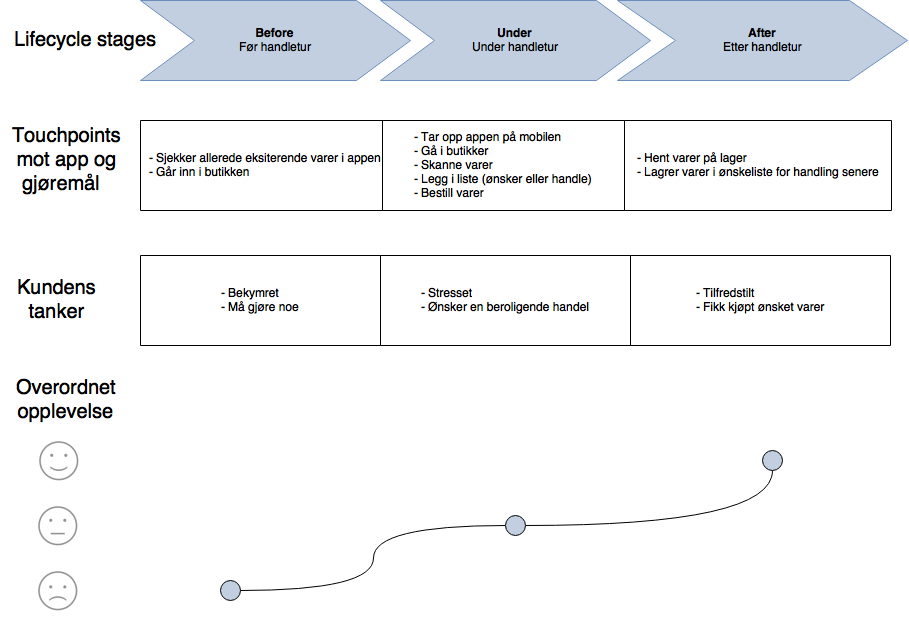
\includegraphics[scale=0.49]{images/customerjourneyBlueprint/cjKunde}
\centering %centering the image
\caption{Kundereise for kunde på Sirkus shopping}
\label{fig:customerKunde}
\end{figure}

\begin{figure}[H]
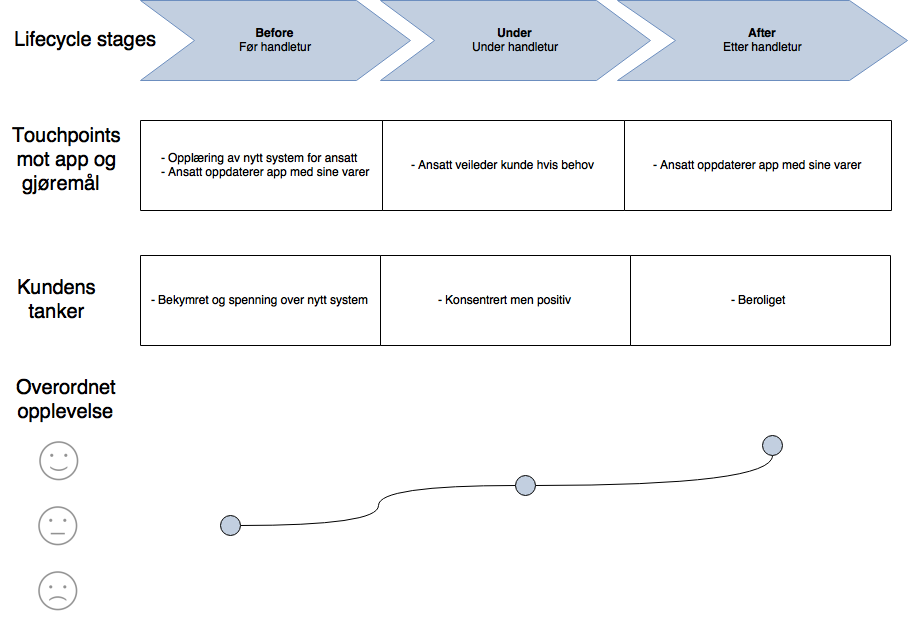
\includegraphics[scale=0.49]{images/customerjourneyBlueprint/cjAnsatt}
\centering %centering the image
\caption{Kundereise for ansatt i butikk på Sirkus shopping}
\label{fig:customerAnsatt}
\end{figure}

\begin{figure}[H]
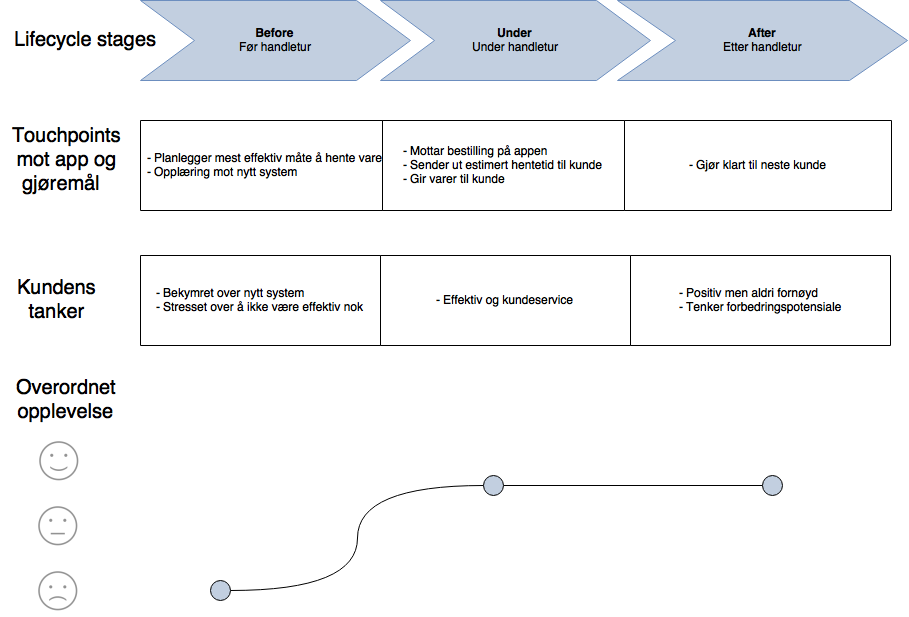
\includegraphics[scale=0.49]{images/customerjourneyBlueprint/cjLager}
\centering %centering the image
\caption{Kundereise for lagerarbeider på Sirkus shopping}
\label{fig:customerLager}
\end{figure}

\subsubsection{Blueprint}
\label{sec:blueprint}
\textit{Blueprint} er en grafisk framstilling av alle aktiviteter som inngår i en tjeneste ved å følge alle personer og komponenter som er involvert og hvordan disse samarbeider for å gjennomføre en prosess\cite{servicedesign}.
Strukturen for et formelt blueprint-diagram er at den inneholder \textit{line of interaction} hvor kunde og media interagerer, \textit{line of visibility} hvor kunden ikke kan se hva som skjer i bakgrunnen og \textit{interaction} hvor business stopper og partnere stepper inn\cite{servicedesign}. I tillegg til dette er de fem p-ene som er snakket om i Service Design 101\cite{101} viktig i en blueprint\cite{servicedesign}. Under er disse presentert, med en berskrivelse av hvordan disse relaterer seg til vårt prosjekt i parentes fra Figur \ref{fig:blueprint}:

\begin{enumerate}
\item \textbf{People}, customers and employees encountered during the prosess. (Kunde, ansatt, lagerabeider)
\item \textbf{Place}, the physical space where the service is delivered. (Sirkus shopping)
\item \textbf{Props}, objects used to produce the service encounter.
\item \textbf{Partners}, other businesses that helps to produce the service.  (Lagerarbeider, systemutviklere)
\item \textbf{Processes}, the workflows that are used to produce the service.  (Effektiv handletur: opplæring blant alle tre aktører, utvikling av brukervennlig applikasjon, kontakt med bankterminal)
\end{enumerate} 

\noindent På bakgrunn av kundereisene fra Kapittel \ref{sec:kundereise}: Kundereiser, lagde gruppen et felles blueprint-diagram, vist i Figur \ref{fig:blueprint}, for disse kundene av applikasjonen. Grunnen til at det ble laget en samlet blueprint var for å tydeliggjøre interaksjonen som skjer mellom kunden på Sirkus shopping, den ansatte, lagerarbeideren og applikasjonen selv. Dette førte til en bedre forståelse av hva som skjer \textit{onstage} og \textit{backstage} i bruk av applikasjonen før, under og etter en handletur på Sirkus shopping. 
\\\\
Symbol 1: Datamaskin = Forespørsel til applikasjon\\
Symbol 2: Krøllalfa = Tilbakemelding fra applikasjon på forspørsel

%Denne bør kanskje legges sidelengs?
\begin{figure}[H]
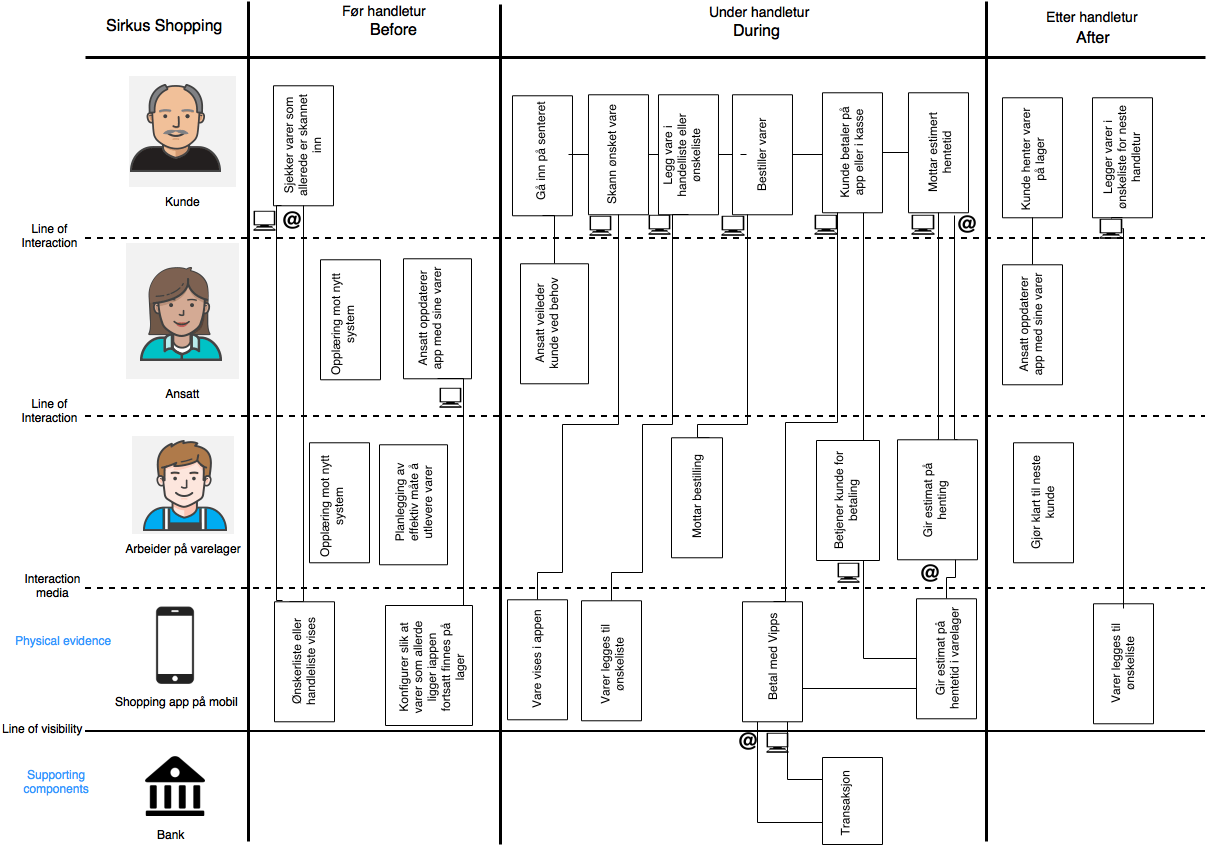
\includegraphics[scale=0.375]{images/customerjourneyBlueprint/blueprint5png}
\caption{Blueprint over handleprosess}
\label{fig:blueprint}
\end{figure}

\subsection{Funksjonelle krav}
\label{funkkrav}
På bakgrunn av ideen gruppen hadde bestemt seg for og analyseringen utført i de ulike tjenestedesign-aktivitetene, ble det utarbeidet en kravspesifikasjon før designet ble påbegynt. Dette ble gjort for å være sikker på at løsningene som ble valgt var gjennomtenkt og at appen ville ha best mulig funksjonalitet. Kravene er listet i Tabell \ref{tab:funksjonelle}.

\begin{table}[H]
    \caption{Funksjonelle krav}
    \label{tab:funksjonelle}
    \centering
    \begin{tabular}{|L{25em} L{18em}|}
    \hline
        \rowcolor[HTML]{D32F2F}
        \textbf{\textcolor{white}{Krav}} & \textbf{\textcolor{white}{Kommentar}}\\
        \rowcolor[HTML]{E6E6E6}
        Applikasjonen skal fungere på smarttelefoner & Gitt av oppgaveteksten\\
        Applikasjonen kan fungere på smartklokker & Gitt av oppgaveteksten
        \\
        \rowcolor[HTML]{E6E6E6}
        Brukeren må kunne logge inn. Da kan brukeren ha tilgang på ønskelistene sine uansett enhet, og dersom man ikke har smarttelefon kan man låne en smarttelefon på senteret og logge inn på denne. Ved å logge inn kan brukeren også dele lister med andre brukere. & Logge inn via e-post. Logge inn via Facebook, gitt av oppgaveteksten. \\ 
        Brukeren må kunne opprette flere ønskelister, slik at man kan sortere varene etter eget ønske. & Mulighet for egendefinere formål med hver ønskeliste\\
        \rowcolor[HTML]{E6E6E6}
        Brukeren må kunne slette ønskelister. & Mulighet for å angre opprettede lister\\
        Brukeren må kunne legge hele ønskelister i handlekurven. & For å forenkle overgangen fra ønskeliste til bestilling av varer\\
        \rowcolor[HTML]{E6E6E6}
        Brukeren må kunne se totalpris på handlekurven i bunn av listen. & Vet prisen på en eventuell bestilling\\
        Brukeren må kunne endre handlekurven. & Kontroll på egen handling\\
        \rowcolor[HTML]{E6E6E6}
        Brukeren må kunne scanne et nytt produkt og legge det til i handlekurv eller liste. & Mulighet for flere produkter inne i app\\
        Brukeren må kunne endre størrelse på produktene. & Kontroll på størrelse på produkter\\
        \rowcolor[HTML]{E6E6E6}
        Brukeren må kunne endre antall av produktene. & Kontroll på antall produkter\\
        Brukeren må kunne navigere fram og tilbake mellom skjermene. & Gode overganger mellom sider, slik at bruker vet hvor han/hun er\\
         \rowcolor[HTML]{E6E6E6}
        Brukeren må kunne betale for handlekurven sin via appen. & Vipps eller tilsvarende\\
        Brukeren skal også kunne betale på senteret, får da beskjed om å henvende seg i skranken & Vet hvor lageret er og får tillit til app\\
        \rowcolor[HTML]{E6E6E6}
        Brukeren må kunne vite hvor lenge det er til han eller hun kan hente varene. & Kan føle tillit til app \\
        Brukeren må kunne dele handlelisten med en venn. & E-post. Facebook.\\
        \rowcolor[HTML]{E6E6E6}
        Appen må være selvmotiverende & Gitt i oppgaveteksten\\
        Appen må ha korrekt innhold & Kan føle seg trygge på at appen er ment for Sirkus shopping\\
        \rowcolor[HTML]{E6E6E6}
        Appen må ha administrator-side for ansatte på varelager & Slik at varelager kan kommunisere med kunde som har bestilt produkter \\
        \hline
    \end{tabular}
\end{table}

\subsection{Ikke-funksjonelle krav}
\label{ikkefunkkrav}

Ikke-funksjonelle krav er vanskelig å måle. De handler ofte om ting som er svært subjektivt. De ikke-funksjonelle kravene i dette prosjektet er listet i Tabell \ref{tab:ikke-funksjonelle}, og det siste er f.eks. at appen må være visuelt tiltrekkende. Dette er svært vanskelig å vurdere, fordi det noe hver og en vurderer individuelt.

\begin{table}[H]
    \caption{Ikke-funksjonelle krav}
    \label{tab:ikke-funksjonelle}
    \centering
    \begin{tabular}{|L{25em} L{18em}|}
    \hline
        \rowcolor[HTML]{D32F2F}
        \textbf{\textcolor{white}{Krav}} & \textbf{\textcolor{white}{Kommentar}}\\
        \rowcolor[HTML]{E6E6E6}
        Appen må være oversiktlig & For at kunder skal forstå \\
        Appen må være intuitiv & For at kunder skal ønske å bruke appen\\
        \rowcolor[HTML]{E6E6E6}
        Appen må være brukbar & Gitt i oppgaveteksten\\
        Appen må være visuelt tiltrekkende & For at kunder skal vise andre og føle trang til å bruke\\
        \hline
    \end{tabular}
\end{table}
